\documentclass[10pt,a4paper,twocolumn]{article}
\usepackage[margin=15mm,top=15mm,bottom=15mm,columnsep=6mm,nohead]{geometry}
\usepackage{amsmath,amssymb}
\usepackage{graphicx}
\usepackage{booktabs}
\usepackage{xcolor}
\usepackage{titlesec}
\usepackage{caption}
\usepackage{float}
\usepackage{fancyhdr}
\usepackage{enumitem}
\usepackage{siunitx}
\usepackage[colorlinks=true,linkcolor=black,citecolor=black,urlcolor=black]{hyperref}

\definecolor{mid}{HTML}{6E6E6E}
\setlength{\parskip}{1.5pt}
\setlength{\parindent}{9pt}
\captionsetup{font=footnotesize,labelfont=bf,skip=2pt}
\titleformat{\section}{\normalsize\bfseries}{\thesection.}{0.4em}{}
\titleformat{\subsection}{\small\bfseries\itshape}{\thesubsection}{0.4em}{}
\titlespacing*{\section}{0pt}{5pt}{2pt}
\titlespacing*{\subsection}{0pt}{3pt}{1pt}
\setlist{itemsep=0pt,topsep=1pt,leftmargin=11pt}
\newcommand{\dfus}{\Delta_{\mathrm{fus}}}
\newcommand{\aoh}{a_{\mathrm{OH}}}
\sisetup{detect-all}
\setlength{\textfloatsep}{8pt plus 2pt minus 2pt}
\setlength{\dbltextfloatsep}{8pt plus 2pt minus 2pt}
\setlength{\floatsep}{6pt plus 2pt minus 2pt}
\setlength{\abovecaptionskip}{3pt}
\renewcommand{\textfraction}{0.08}
\renewcommand{\topfraction}{0.95}
\renewcommand{\dbltopfraction}{0.95}
\renewcommand{\floatpagefraction}{0.9}
\renewcommand{\dblfloatpagefraction}{0.9}

\pagestyle{plain}

\begin{document}

\twocolumn[
\begin{center}
{\Large\bfseries The Ice Decides\par
Solid--liquid equilibrium for freeze concentration\par
and cryoprotectant design\par}\vspace{8pt}
{\normalsize Siddhant Chowdhary (25B0347)\par}\vspace{1pt}
{\small Theme: Thermodynamics in Biological Systems\par}
\end{center}
\vspace{-2pt}
\begin{quote}\small
\textbf{Abstract.} Cryopreservation banks blood, cells and tissues. Better methods could one day store
organs for transplant. Each new protectant recipe is still found by measurement. Slow freezing concentrates
salt around and inside cells. Because ice is pure water, solid--liquid equilibrium fixes the water activity of
every liquid touching ice. A recipe changes only how much water stays liquid
and which solutes share it. To predict this without measuring every mixture, we model water activity with one
constant per hydroxyl group, fitted on glycerol alone and tested blind. It predicted
ethylene glycol, sucrose and maltose 3--17$\times$ more accurately than an ideal solution and beat UNIFAC for
every solute except sorbitol. For glycerol\,+\,NaCl above 30\,wt\% solute it was 3--5$\times$ more accurate
than two standard cryobiology models. It fails for sorbitol and simple alcohols. Sucrose at two temperatures
traces this to the molecule and gives an interaction enthalpy of $-6$ to $-8$\,kJ\,mol$^{-1}$ per OH. The
model shows that non-penetrating
sorbitol lowers salt outside a cell but not inside. Whether it spares glycerol depends on the injury
mechanism. Under three literature criteria it saves 0.76\,g glycerol per gram, costs 2.1\,g or allows an
11\% reduction.
\end{quote}
\vspace{2pt}
]

%===================================================================== INTRODUCTION
\section{Introduction and background}

\textbf{Why it matters.} Freezing is how blood, sperm, embryos and stem cells are banked. Better preservation
of cells, tissues and whole organs would ease limits on transplantation, regenerative medicine and drug
discovery \cite{giwa}. Every protectant recipe is a compromise. Too little and salt or ice injures the cells.
Too much and the protectant itself is toxic. Today each recipe is tuned by experiment, which is slow and
costly.

\textbf{Problem.} In slow freezing, ice forms outside the cells first. The unfrozen solution concentrates and water leaves the cells. This solution
injury, one arm of Mazur's two-factor account of freezing damage \cite{mazur}, acts between $-15$ and
$-60$\,\textdegree C \cite{gao}. Lovelock showed
that glycerol protects red cells by diluting the salt that would otherwise accumulate \cite{lovelock10,lovelock11}.
Mazur later found that the amount of liquid left matters as much as its salt content \cite{mazur81,mazur89}.
In Pegg's words, ``Cryoprotectants, simply by increasing the total concentration of all solutes in the system,
reduce the amount of ice formed at any given temperature; but to be biologically acceptable they must be able
to penetrate into the cells and have low toxicity'' \cite{pegg}. The first half of that sentence is
thermodynamics. This work makes the second half quantitative too.

\textbf{Thermodynamic principle.} At equilibrium the chemical potential of water is the same in ice and in
the liquid. Ice is pure, so $\mu_w^{\mathrm{ice}}(T)=\mu_w^{\mathrm{L}}(T)+RT\ln(x_w\gamma_w)$, which means
$RT\ln(x_w\gamma_w)=-\dfus G(T)$. Since $G$ is a state function, $\dfus G(T)$ can be evaluated along a
heat--melt--cool path through $T_m$ \cite{sandler},
\begin{equation*}
\begin{split}
\dfus H(T)&=\dfus H+\Delta C_p(T-T_m),\\
\dfus S(T)&=\dfus H/T_m+\Delta C_p\ln(T/T_m),
\end{split}
\end{equation*}
and $\dfus G=\dfus H(T)-T\dfus S(T)$ gives
\begin{equation}
\begin{split}
\ln(x_w\gamma_w) = &-\frac{\dfus H}{R}\Big(\frac1T-\frac1{T_m}\Big)\\
&-\frac{\Delta C_p}{R}\Big(\frac{T_m}{T}-1+\ln\frac{T}{T_m}\Big)
\end{split}
\label{eq:sle}
\end{equation}
with $\dfus H=\SI{6009.5}{J\,mol^{-1}}$, $\Delta C_p=\SI{37.9}{J\,mol^{-1}K^{-1}}$ and $T_m=273.15$\,K. The
right-hand side depends on $T$ only, which has two consequences used throughout. (i) Once ice is present, the
water activity $a_w$ of the unfrozen liquid is fixed by temperature. Additives cannot change it. They change
only how much water must freeze out to reach it. (ii) A cell at osmotic equilibrium has the same $a_w$ inside,
so its intracellular salt is set by which solutes can enter it. Everything else hinges on $\gamma_w$. For
water--polyol mixtures $\gamma_w<1$ because hydroxyl groups hydrogen-bond to water. A polyol therefore lowers
the freezing point more than Raoult's law predicts.

\begin{figure}[t]
\centering
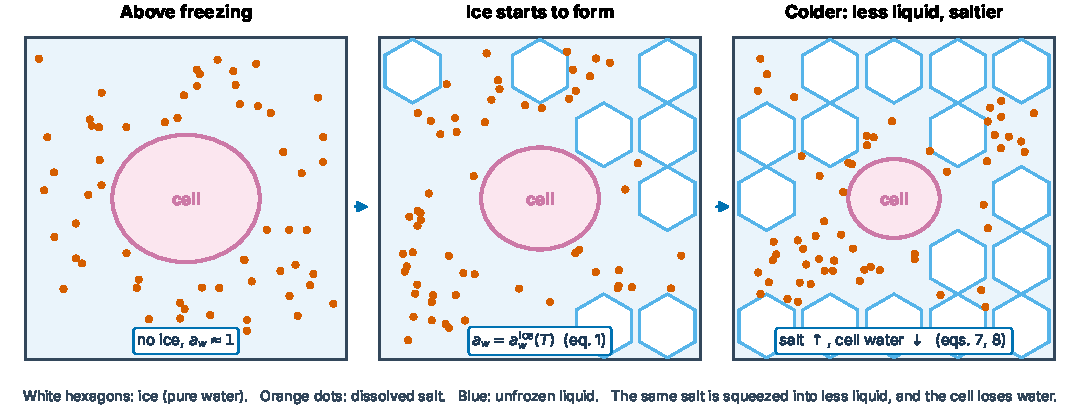
\includegraphics[width=\columnwidth]{fig_freeze_concentration.pdf}
\caption{Freeze concentration. Ice is pure water, so the same solutes are squeezed into less liquid as $T$
falls and water leaves the cell.}
\label{fig:schematic}
\end{figure}

\textbf{Existing approaches.} Cryobiology uses ideal-dilute models, the osmotic virial equation
\cite{elliott,zielinski} and freezing-point summation \cite{km}. The last two need coefficients fitted for every
solute. Empirical phase-diagram equations exist for water--glycerol--NaCl \cite{fahy}, measured by thermal
analysis \cite{shepard}. Margules models have been fitted to water--glycerol SLE \cite{zargarzadeh}, so a glycerol
fit alone is not new. Group-contribution methods (UNIFAC \cite{unifac}, Dortmund \cite{dortmund}) predict any
molecule from parameters fitted mostly to vapour--liquid data. Polyol- and sugar-specific versions exist at
25\,\textdegree C \cite{marcolli,peres}. A recent review suggests such models could screen cryoprotectant
mixtures but does not apply them to freezing \cite{powellpalm}.

\textbf{Why a predictive model.} Every existing route to the freeze concentration of a new recipe starts with
measurements. Either a phase diagram is measured for that mixture (Shepard \emph{et al.}\ needed nine
composition series by thermal analysis for one ternary system \cite{shepard}) or freezing data are needed for
every solute before the summation or virial models can be used. Screening candidate formulations this way
multiplies experiments. We therefore set three design criteria for the method itself. Cost means no new
measurements to make a prediction, since the single parameter comes from published glycerol data. Time means a
prediction is one root-finding step on a laptop and the whole study is rebuilt by one command. Feasibility
means the inputs are textbook properties of ice, the number of OH groups and one constant, while validation
needs only a few samples with calibrated temperature probes (Section~\ref{sec:val}).

\textbf{Gap, hypothesis and contributions.} Per-solute coefficients cannot be used for unmeasured molecules.
General group parameters are not tuned to freezing. Our hypothesis is that one water--OH constant, fitted on
glycerol only, predicts the freezing of other polyols and of polyol\,+\,salt mixtures without refitting. We
test it blind against 13 solutes, two solutes at 25\,\textdegree C and a ternary phase diagram, using
cryobiology's own models as benchmarks. We then diagnose where and why it fails, including an
enthalpy--entropy split of the interaction. Finally we use it to show how freeze concentration acts inside
and outside a cell and what that implies for glycerol-sparing recipes. This combination was not found in the literature we searched.

%===================================================================== METHODS
\section{Methodology}

\begin{figure*}[t]
\centering
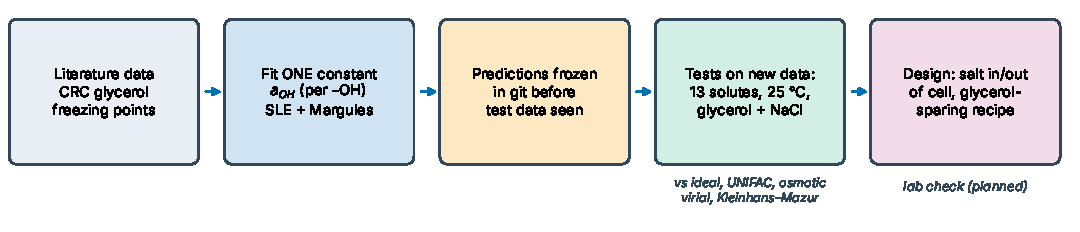
\includegraphics[width=0.86\textwidth]{report_pipeline.pdf}
\caption{Workflow. One constant is fitted on glycerol, frozen in version control and tested against data it
has never seen. Only then is it used for design. Every figure and table is rebuilt by one command
(\texttt{run\_all.py}).}
\label{fig:pipeline}
\end{figure*}

\subsection{Thermodynamic framework}
Every calculation is eq.~(\ref{eq:sle}) with a model for $\ln a_w$ of the liquid, solved numerically for the
unknown ($T$ or the amount of water left liquid).

\emph{Polyols.} Only water--solute pair interactions are kept, as a one-constant Margules term for each solute
proportional to its number of OH groups
\begin{equation}
\frac{G^{\mathrm{ex}}}{RT}=x_w\sum_i\alpha_i x_i,\qquad \alpha_i=\frac{n_{\mathrm{OH},i}\,\aoh}{RT}.
\label{eq:model}
\end{equation}
Differentiating $nG^{\mathrm{ex}}$ gives the activity coefficients
\begin{equation}
\begin{split}
\ln\gamma_w&=(1-x_w)\textstyle\sum_i\alpha_i x_i,\\
\ln\gamma_i&=\alpha_i x_w-x_w\textstyle\sum_j\alpha_j x_j ,
\end{split}
\label{eq:gamma}
\end{equation}
which satisfy Gibbs--Duhem, $x_w\,\mathrm{d}\ln\gamma_w+\sum_i x_i\,\mathrm{d}\ln\gamma_i=0$ (numerical residual
$\sim10^{-14}$). Glycerol has 3 OH groups, ethylene glycol 2, sorbitol 6 and sucrose 8.

\emph{Salt.} NaCl ($\nu=2$) enters through an osmotic coefficient fitted to its CRC ice line \cite{crc} with
RMSE 0.023\,K to the eutectic. Its first term has the Debye--H\"uckel shape.
\begin{equation}
\ln a_w^{\mathrm{NaCl}}=-\nu mM_w\phi(m),\;\; \phi=1-\frac{a\sqrt m}{1+\sqrt m}+bm+cm^2
\label{eq:salt}
\end{equation}

\emph{Mixtures.} Contributions are added in $\ln a_w$ with no salt--polyol cross term
\begin{equation}
\begin{split}
\ln a_w&=\ln x_w+(1-x_w)\textstyle\sum_i\alpha_i x_i\;-\;\nu\,m\,M_w\,\phi(m)\\
&=\ln a_w^{\mathrm{ice}}(T),
\end{split}
\label{eq:mix}
\end{equation}
where $x$ runs over water and polyols and $m$ is per kg water. This rule follows from the activity framework
and was fixed before mixture data were seen. Summing freezing-point depressions \cite{km} is reported only as a
comparison. In the dilute limit eq.~(\ref{eq:mix}) reduces to $\Delta T=K_f\sum_j\nu_jm_j$ with
$K_f=RT_m^2M_w/\dfus H=1.86$\,K\,kg\,mol$^{-1}$, which checks the constants.

\emph{Fit.} $\aoh$ was fitted by least squares to 19 CRC glycerol freezing points between 2 and 40\,wt\%
\cite{crc} by solving eqs.~(\ref{eq:sle}) and (\ref{eq:gamma}) for $T$. The result is
$\aoh=-2414.9$\,J\,mol$^{-1}$ (bootstrap 95\% interval $-2461$ to $-2395$, data scatter only). The interaction
energy was assumed independent of $T$, so $\alpha_i\propto1/T$. This was fixed before any test at another
temperature.

\emph{Diagnostics.} Away from ice, isopiestic data give the osmotic coefficient
$\phi=-\ln a_w/(M_w\sum_j\nu_jm_j)$. Any measured $a_w$ can be inverted for the constant a molecule implies,
$a=RT\,(\ln a_w-\ln x_w)/(n_{\mathrm{OH}}x_s^2)$. Its temperature dependence can be split by Gibbs--Helmholtz
\begin{equation}
a(T)=h-Ts,\qquad h=\frac{\partial(a/T)}{\partial(1/T)},
\label{eq:gh}
\end{equation}
where $h$ and $s$ are the enthalpy and entropy of the water--OH interaction.

\subsection{Blind tests and benchmarks}
After the fit, predictions were committed to a git repository and never edited. Test data were entered only
afterwards. Single solutes were CRC freezing points for ethylene glycol, mannitol, glucose, fructose, sucrose
and four alcohols \cite{crc}, then maltose and lactose in a later round \cite{crc}, plus sorbitol by DSC at
53--64\,wt\% \cite{siniti}. A cryoscope sorbitol set \cite{baer} was excluded because it implied
$\phi\approx1.14$ at 1\,wt\%, where $\phi$ must approach 1. At another temperature we used isopiestic data at
25\,\textdegree C for sorbitol \cite{bower} and sucrose \cite{robinson}. For mixtures we used the
water--glycerol--NaCl liquidus \cite{shepard}. It is published only as a figure, so it was digitised by hand
(nine glycerol to NaCl ratios, 76 points) with the calibration checked against the NaCl--water eutectic. The
pass criterion fixed in advance was RMS $\le0.5$\,K for total solute $\le30$\,wt\%. Benchmarks were the ideal
solution, UNIFAC and Dortmund \cite{unifac,dortmund,thermo} and for mixtures the osmotic virial equation and the
Kleinhans--Mazur summation with published coefficients \cite{zielinski,km}.

\subsection{Freeze concentration inside and outside a cell}
A medium of water $W_0$ and solutes $n_j$ (0.9\,wt\% NaCl plus additives) is cooled below its freezing point.
Solutes stay in the liquid, so a fraction $\varphi$ of the water freezes until
\begin{equation}
\ln a_w\big(\{n_j\},\,(1-\varphi)W_0\big)=\ln a_w^{\mathrm{ice}}(T),
\label{eq:balance}
\end{equation}
with $\ln a_w$ from eq.~(\ref{eq:mix}) and the right-hand side from eq.~(\ref{eq:sle}). A cell at osmotic
equilibrium (slow cooling) has the same $a_w$ inside. Its own solutes $n_c$ are represented as isotonic NaCl.
Glycerol penetrates at the external molality $m_g(T)$ while sorbitol and NaCl are excluded. The cell water
$W_c$ then solves
\begin{equation}
\ln a_w\big(n_c/W_c,\;m_g(T)\big)=\ln a_w^{\mathrm{ice}}(T).
\label{eq:cell}
\end{equation}
Recipes are designed at $-15$\,\textdegree C \cite{gao} under three criteria from the literature. The first is
NaCl outside the cell $\le4.41$\,wt\%, the onset of red-cell haemolysis \cite{lovelock11,shepard}. The second
is the same limit inside the cell. The third is unfrozen water $\ge25\%$, above which most red cells survived
regardless of salt \cite{mazur81}. For each criterion we report the sparing ratio $-\mathrm{d}w_g/\mathrm{d}w_s$,
the glycerol saved per gram of sorbitol.

\subsection{Proposed experimental validation}\label{sec:val}
Laboratory access was not available before submission, so the experiment is proposed with its predictions
already committed. The available reagents (NaCl and glycerol) are enough. Freezing points would come from
cooling curves with calibrated probes in an ice--NaCl bath (to about $-18$\,\textdegree C, above the
$-21.1$\,\textdegree C eutectic), taking the post-recalescence maximum corrected for supercooling. This follows
the thermal-analysis approach of \cite{shepard} and the re-measurement strategy of \cite{benson}. Samples and
committed predictions are in Table~\ref{tab:lab}. An uncertainty budget (probe calibration, nonlinearity,
weighing, purity, supercooling and repeatability) gives $\pm0.25$\,K at 95\%. That is enough to resolve our
model from the ideal one (0.7--1.3\,K apart) but not the three mixing rules (0.2--0.7\,K).

\begin{table}[t]
\centering\footnotesize\setlength{\tabcolsep}{3pt}
\caption{Proposed validation. Committed predictions of the freezing point (\textdegree C).}
\label{tab:lab}
\begin{tabular}{@{}lcccc@{}}
\toprule
Sample (wt\%) & Per-OH & Ideal gly. & K--M & Osm.\ virial\\
\midrule
NaCl 5 (standard) & \multicolumn{4}{c}{CRC $-3.05$}\\
Glycerol 30 (standard) & $-9.69$ & $-7.87$ & -- & --\\
Glycerol 20 + NaCl 5 & $-9.42$ & $-8.68$ & $-9.69$ & $-9.92$\\
Glycerol 25 + NaCl 5 & $-11.71$ & $-10.45$ & $-12.11$ & $-12.42$\\
\bottomrule
\end{tabular}
\end{table}

%===================================================================== RESULTS
\section{Results and discussion}

\begin{figure*}[t]
\centering
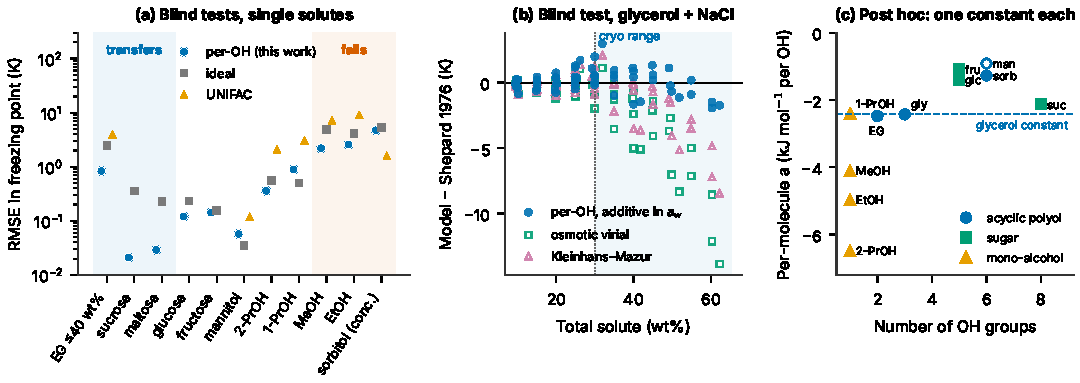
\includegraphics[width=\textwidth]{report_results_v2.pdf}
\caption{(a) Freezing-point error on single solutes not used in the fit (log scale). The blue band marks
molecules where the constant transfers and the red band where it fails. (b) Error on the
water--glycerol--NaCl liquidus \cite{shepard}. All three models predict from single-solute data. (c) Post hoc
constant each molecule would need on its own (fits $\le20$\,wt\%). Open symbols mark depressions below 3\,K,
where the constant is weakly determined. The dashed line is the glycerol constant used in the blind tests.}
\label{fig:results}
\end{figure*}

\begin{table*}[t]
\centering\footnotesize\setlength{\tabcolsep}{4pt}
\caption{Blind tests (error = model $-$ data, RMSE in K unless stated). $\aoh$ was never refitted.}
\label{tab:results}
\begin{tabular}{@{}llccccl@{}}
\toprule
Test & Data & Per-OH & Ideal & UNIFAC & Other & Verdict\\
\midrule
Glycerol (fit) & CRC \cite{crc} & 0.02 & 1.31 & 2.1 & 0.27$^a$ & fit\\
Ethylene glycol, 2--40\,wt\% & CRC & \textbf{0.83} & 2.49 & 3.99 & 0.52$^a$ & transfers\\
Sucrose, to 40\,wt\% & CRC & \textbf{0.02} & 0.35 & -- & 0.02$^a$ & transfers\\
Maltose, to 40\,wt\% (later round) & CRC & \textbf{0.03} & 0.23 & -- & -- & transfers\\
Glucose / fructose & CRC & 0.12/0.14 & 0.23/0.15 & -- & 0.01/--$^a$ & weak test\\
MeOH / EtOH & CRC & 2.20/2.57 & 4.84/4.12 & 7.2/9.1 & 1.29/0.91$^a$ & fails\\
Sorbitol, 53--64\,wt\% & DSC \cite{siniti} & 4.7 & 5.3 & \textbf{1.6} & -- & fails\\
Sorbitol 25\,\textdegree C (RMS in $\phi$) & isopiestic \cite{bower} & 0.163 & \textbf{0.060} & 0.113 & -- & fails\\
Glycerol\,+\,NaCl, $\le$30\,wt\% solute & digitised \cite{shepard} & 0.69 & 0.89$^b$ & -- & 0.69$^a$/0.59$^c$ & misses 0.5\,K target\\
Glycerol\,+\,NaCl, $>$30\,wt\% solute & digitised \cite{shepard} & \textbf{1.23} & 4.64$^b$ & -- & 5.75$^a$/3.39$^c$ & best\\
\bottomrule
\end{tabular}\\[1pt]
{\scriptsize $^a$Osmotic virial \cite{zielinski}, fitted per solute (in-sample for single solutes). $^b$Ideal glycerol\,+\,fitted NaCl. $^c$Kleinhans--Mazur summation \cite{km}.}
\end{table*}

\begin{figure}[t]
\centering
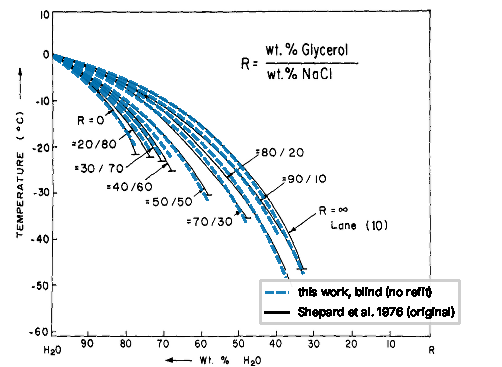
\includegraphics[width=\columnwidth]{shepard_overlay.pdf}
\caption{Water--glycerol--NaCl liquidus isopleths reproduced from Shepard \emph{et al.}\ \cite{shepard}
(Fig.~3, black) with this work's blind predictions drawn on top (blue dashed). Only the glycerol-only curve
($R=\infty$) corresponds to the data used in the fit.}
\label{fig:shepard}
\end{figure}

\subsection{Where one constant per OH holds}
For ethylene glycol, glycerol, sucrose and maltose a constant fitted on glycerol predicts freezing without
refitting and does as well as osmotic virial coefficients fitted to each molecule (Table~\ref{tab:results},
Fig.~\ref{fig:results}a). Lactose dissolves only to 8\,wt\%, which is too dilute to discriminate.
Fig.~\ref{fig:shepard} draws the blind predictions over Shepard's original phase diagram. On this liquidus the
model missed the pre-set 0.5\,K target at low concentration (0.69\,K). There the digitised figure is itself
uncertain by 0.34\,K (its pure-glycerol and pure-NaCl edges against CRC) and all three mixture models agree
within 0.1\,K. Above 30\,wt\% solute, which are the conditions cells meet during freezing, adding $\ln a_w$ is
about 3$\times$ more accurate than the cryobiology models (Fig.~\ref{fig:results}b). Isopiestic
sorbitol\,+\,NaCl data \cite{bower} show why. The neglected salt--polyol cross term (salting-in) is 0.6--5\% of
the osmolality, or 0.05--0.13\,K at recipe conditions. A virial-type cross coefficient would remove this, but
it needs ternary data for every salt--polyol pair, which is the per-mixture measurement this method avoids.
With the error under a fifth of the model's own, the additive rule is the better choice for screening. A cross
term is worth adding only to refine a final recipe.

\begin{figure*}[t]
\centering
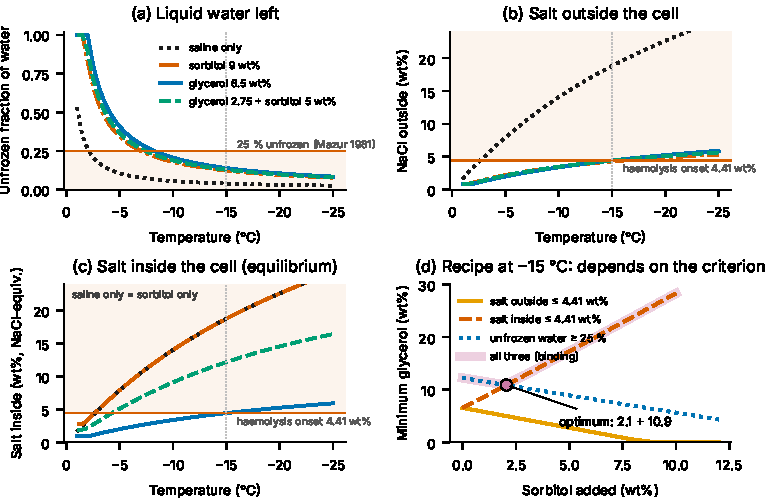
\includegraphics[width=0.68\textwidth]{freeze_concentration_cells.pdf}
\caption{Freeze concentration in 0.9\,wt\% saline with the per-OH model. (a) Unfrozen fraction of the water.
(b) NaCl in the unfrozen medium. (c) Salt inside a cell at osmotic equilibrium. Glycerol penetrates and
sorbitol does not, so the saline-only and sorbitol-only curves coincide. (d) Minimum glycerol at
$-15$\,\textdegree C against sorbitol added under three literature criteria. The purple band shows all three
at once with its optimum.}
\label{fig:cells}
\end{figure*}

\begin{figure*}[t]
\centering
\begin{minipage}[t]{0.45\textwidth}\centering
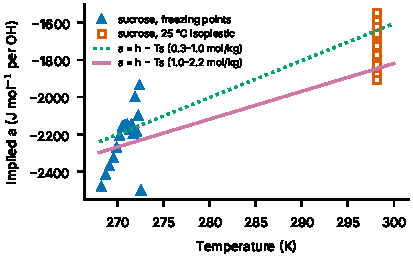
\includegraphics[width=0.86\linewidth]{posthoc_gibbs_helmholtz.pdf}
\caption{Post hoc per-OH constant implied by sucrose data near 0\,\textdegree C and at 25\,\textdegree C, with
$a=h-Ts$ fitted on two matched molality windows.}
\label{fig:gh}
\end{minipage}\hfill
\begin{minipage}[t]{0.45\textwidth}\centering
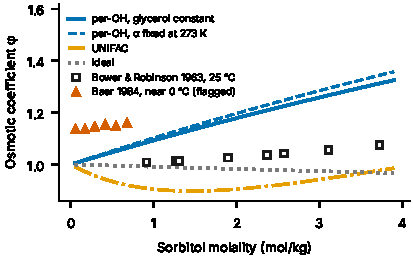
\includegraphics[width=0.86\linewidth]{sorbitol_25C_phi.pdf}
\caption{Sorbitol at 25\,\textdegree C \cite{bower}. With glycerol's constant the per-OH model overstates
non-ideality. An older freezing-point set \cite{baer} is implausible at infinite dilution, where $\phi$ must
tend to 1.}
\label{fig:sorbitol}
\end{minipage}
\end{figure*}

\subsection{Where it fails and what the failure teaches}
The model overstates sorbitol's non-ideality by 3.5--5.5\,K when concentrated and four- to five-fold in
$\phi-1$ at 25\,\textdegree C (Fig.~\ref{fig:sorbitol}). Two causes were possible and sucrose separates them.
On the freezing line sucrose implies $a\approx-2200$\,J\,mol$^{-1}$ per OH, close to glycerol's. At
25\,\textdegree C it implies about $-1800$. Sorbitol at the same 25\,\textdegree C implies only $-400$ to $-750$. The failure
is mainly the molecule. Post hoc (after the blind tests), letting each molecule have its own constant shows a
pattern (Fig.~\ref{fig:results}c). Short acyclic polyols sit at $\approx-2.4$\,kJ\,mol$^{-1}$ while six-OH
chains (mannitol, sorbitol) fall to $-0.9$ to $-1.3$. Adjacent hydroxyls on a flexible chain can bond to each
other rather than to water, so counting them independently overstates their pull on water. A proximity
correction of this kind is used for sugars \cite{peres}. The simplest version subtracts a term per pair of OH
groups on neighbouring carbons, $A_i=n_{\mathrm{OH},i}\aoh-n_{\mathrm{pair},i}\,\delta$. The post hoc constants
already show it cannot be adjacency alone. Ethylene glycol and glycerol (0.50 and 0.67 neighbouring pairs per
OH) share $a\approx-2.45$\,kJ\,mol$^{-1}$ while sorbitol (0.83) needs $-1.3$, so chain length or conformation
must enter. A $\delta$ fitted to sorbitol would remove its deviation by construction, so we do not claim it.
The test is xylitol, maltitol and lactitol \cite{uraji}, whose blind predictions are committed.


\emph{Gibbs--Helmholtz split (post hoc, Fig.~\ref{fig:gh}).} Applying eq.~(\ref{eq:gh}) to sucrose at both
temperatures over matched molality windows gives $h=-6.3$ to $-7.6$\,kJ\,mol$^{-1}$ and $s=-15$ to
$-20$\,J\,mol$^{-1}$K$^{-1}$ per OH. The water--OH interaction is strongly exothermic, consistent with hydrogen
bonding. It is partly offset by an entropy loss as water is ordered around the solute. Because $|Ts|$ grows
with $T$ the net attraction weakens on warming. This is why the constant-energy assumption ($\alpha\propto1/T$)
overstates non-ideality at 25\,\textdegree C and why our freezing-line fit should not be used for
room-temperature water activity.

\textbf{Ours versus UNIFAC.} UNIFAC's many group parameters were fitted mostly to vapour--liquid data at and
above room temperature. For water--glycerol it gives the wrong sign ($\gamma_w>1$) and misses the depression by
up to about 6\,K at 40\,wt\%. One group and one constant fitted on freezing data trade breadth for accuracy
within one class of molecules.



\subsection{What freeze concentration does inside the cell}
Without a cryoprotectant the unfrozen medium of saline holds 18.8\,wt\% NaCl at $-15$\,\textdegree C and only
3.9\% of the water is still liquid (Fig.~\ref{fig:cells}a,b). Glycerol 6.5\,wt\% or sorbitol 9\,wt\% each bring
the salt outside the cell down to the 4.41\,wt\% haemolysis limit. Inside the cell they differ completely
(Fig.~\ref{fig:cells}c). Glycerol enters the cell, shares the osmotic load and keeps intracellular salt at
4.4\,wt\%. Sorbitol stays outside, so the cell's interior still contains only its own salts. These must reach
the $a_w$ set by the ice, which gives 18.8\,wt\%, the same as in plain saline. This is consequence (ii) of
eq.~(\ref{eq:sle}) and it turns Pegg's ``must penetrate'' \cite{pegg} into a number.

\textbf{Design depends on the injury mechanism} (Fig.~\ref{fig:cells}d). If injury comes from salt outside the
cell \cite{lovelock11}, sorbitol spares 0.76\,g of glycerol per gram. This holds across three activity models
(0.68--0.91\,g/g, $\pm25\%$ salt limit, $-10$ to $-20$\,\textdegree C). If it comes from salt inside, sorbitol
costs 2.1\,g of glycerol per gram, because it keeps more water liquid outside and so dilutes the glycerol that
must enter the cell. If it comes from too little liquid \cite{mazur81}, sorbitol helps (0.66\,g/g). Requiring
all three at once gives an interior optimum of 2.1\,wt\% sorbitol with 10.9\,wt\% glycerol, 11\% less glycerol
than glycerol alone (12.2\,wt\%). Mazur's experiments suggest that which criterion dominates depends on cell
concentration and on how much water freezes \cite{mazur81,mazur89}. The model makes that trade-off explicit.
For red cells cooled slowly in saline to $-15$\,\textdegree C, sorbitol is worth adding only up to about
2\,wt\%, beyond which the cell interior becomes the weak point.

\textbf{Scope.} The results are equilibrium predictions. They assume slow cooling and model the cell's solutes
as isotonic NaCl. Cooling-rate kinetics, intracellular ice and toxicity are not included. The model predicts
the conditions a cell experiences, not whether it survives.

%===================================================================== CONCLUSION
\section{Conclusion and next steps}

A single hydroxyl constant fitted on one molecule predicts the freezing of small polyols, sucrose, maltose and
glycerol\,+\,salt mixtures without refitting. It matches per-molecule cryobiology models when dilute and beats
them when concentrated. It fails for six-OH chains and simple alcohols. These failures are diagnostic. The post
hoc constants point to neighbouring-OH interactions and the sucrose data split the interaction into a
hydrogen-bond enthalpy and an ordering entropy. Because ice fixes water activity everywhere, a non-penetrating
additive cannot protect a cell's interior. Whether it spares glycerol depends on which injury mechanism
dominates. The model puts a number on each case. In practice this is a cheap and fast screen. Recipes are
ranked from textbook data and one constant. The laboratory is needed only to confirm the chosen few and for
molecules such as six-OH chains where the screen fails.

\textbf{Next steps.} (1) Run the proposed validation (Section~\ref{sec:val}). (2) Add a hydroxyl-proximity term
and test it on xylitol, maltitol and lactitol. (3) Check $h$ against calorimetric mixing enthalpies. (4) Couple
the framework to membrane transport for finite cooling rates. In the two-parameter model \cite{kleinhans2p}
cell water and glycerol follow
$\mathrm{d}V_w/\mathrm{d}t=L_pA\,(RT/\bar V_w)\ln(a_w^{\mathrm{out}}/a_w^{\mathrm{in}})$ and
$\mathrm{d}n_g/\mathrm{d}t=P_sA\,(c_g^{\mathrm{out}}-c_g^{\mathrm{in}})$, with $a_w^{\mathrm{out}}$ from
eq.~(\ref{eq:sle}) at each instant of cooling and $a_w^{\mathrm{in}}$ from eq.~(\ref{eq:mix}). This replaces
the dilute osmolality of the classical treatment \cite{mazur63} with the non-ideal activity. That matters most
when the cell is most dehydrated.

{\footnotesize\textbf{Code and data.} Models, data with sources, committed predictions and all analyses are at
\url{https://github.com/Siddhant-Chowdhary/Thermodynamics-Project-}. The README maps every figure and table to
its script. \texttt{python run\_all.py} rebuilds them all and \texttt{run\_in\_colab.ipynb} runs the same
pipeline in a browser. An interactive version (\texttt{app.py}, online at
\url{https://the-ice-decides.streamlit.app}) lets a reader pick a recipe and a temperature and see the unfrozen
water and the salt inside and outside the cell.\par}

\renewcommand{\refname}{\normalsize\bfseries References}
\begin{thebibliography}{99}
\scriptsize
\setlength{\itemsep}{-1.2pt}\setlength{\parsep}{0pt}
\bibitem{mazur} P. Mazur, \emph{Am.\ J.\ Physiol.} 247 (1984) C125.
\bibitem{giwa} S. Giwa et al., \emph{Nat.\ Biotechnol.} 35 (2017) 530.
\bibitem{gao} D. Gao, J.\,K. Critser, \emph{ILAR J.} 41 (2000) 187.
\bibitem{lovelock10} J.\,E. Lovelock, \emph{Biochim.\ Biophys.\ Acta} 10 (1953) 414.
\bibitem{lovelock11} J.\,E. Lovelock, \emph{Biochim.\ Biophys.\ Acta} 11 (1953) 28.
\bibitem{mazur81} P. Mazur, W.\,F. Rall, N. Rigopoulos, \emph{Biophys.\ J.} 36 (1981) 653.
\bibitem{mazur89} P. Mazur, K.\,W. Cole, \emph{Cryobiology} 26 (1989) 1.
\bibitem{pegg} D.\,E. Pegg, \emph{Methods Mol.\ Biol.} 368 (2007) 39.
\bibitem{sandler} S.\,I. Sandler, \emph{Chemical, Biochemical, and Engineering Thermodynamics}, 4th ed., Wiley, 2006.
\bibitem{elliott} J.\,A.\,W. Elliott et al., \emph{J.\ Phys.\ Chem.\ B} 111 (2007) 1775.
\bibitem{zielinski} M.\,W. Zielinski et al., \emph{Cryobiology} 69 (2014) 305.
\bibitem{km} F.\,W. Kleinhans, P. Mazur, \emph{Cryobiology} 54 (2007) 212.
\bibitem{fahy} G.\,M. Fahy, \emph{Biophys.\ J.} 32 (1980) 837.
\bibitem{shepard} M.\,L. Shepard, C.\,S. Goldston, F.\,H. Cocks, \emph{Cryobiology} 13 (1976) 9.
\bibitem{zargarzadeh} L. Zargarzadeh, J.\,A.\,W. Elliott, \emph{J.\ Phys.\ Chem.\ B} 123 (2019) 1099.
\bibitem{unifac} Aa. Fredenslund, R.\,L. Jones, J.\,M. Prausnitz, \emph{AIChE J.} 21 (1975) 1086.
\bibitem{dortmund} U. Weidlich, J. Gmehling, \emph{Ind.\ Eng.\ Chem.\ Res.} 26 (1987) 1372.
\bibitem{marcolli} C. Marcolli, Th. Peter, \emph{Atmos.\ Chem.\ Phys.} 5 (2005) 1545.
\bibitem{peres} A.\,M. Peres, E.\,A. Macedo, \emph{Fluid Phase Equilib.} 139 (1997) 47.
\bibitem{powellpalm} M.\,J. Powell-Palm, A.\,N. Consiglio, arXiv:2601.12573 (2026).
\bibitem{thermo} C. Bell et al., \emph{thermo} (Python package) v0.6.1, \url{https://github.com/CalebBell/thermo}.
\bibitem{crc} D.\,R. Lide (ed.), \emph{CRC Handbook of Chemistry and Physics}, Internet Version 2005, pp.\ 8-58 to 8-84.
\bibitem{siniti} M. Siniti, S. Jabrane, J.\,M. L\'etoff\'e, \emph{Thermochim.\ Acta} 325 (1999) 171.
\bibitem{baer} R.\,J. Baer, K.\,A. Baldwin, \emph{J.\ Dairy Sci.} 67 (1984) 2860.
\bibitem{bower} V.\,E. Bower, R.\,A. Robinson, \emph{J.\ Phys.\ Chem.} 67 (1963) 1540.
\bibitem{robinson} R.\,A. Robinson, R.\,H. Stokes, \emph{Trans.\ Faraday Soc.} 45 (1949) 612.
\bibitem{uraji} T. Uraji et al., \emph{Food Sci.\ Technol.\ Int.} 2 (1996) 38.
\bibitem{mazur63} P. Mazur, \emph{J.\ Gen.\ Physiol.} 47 (1963) 347.
\bibitem{kleinhans2p} F.\,W. Kleinhans, \emph{Cryobiology} 37 (1998) 271.
\bibitem{benson} J.\,D. Benson et al., \emph{Cryobiology} 61 (2010) 352.
\end{thebibliography}

\end{document}
